In this section there aren't mockups showing the design of the mobile apps because they have already been inserted in the RASD but there are mockups representing the third parties' desktop application.\\
After a reasonable analysis of the real world in which the final product will be insert, the third parties' app has been designed as a multichannel application . Third parties are companies, no profit societies, govarnement offices so it is reasonable to think that the main way to access to the app is via one or more desktops inside them; it has been chosen to add also the mobile version to obtain a larger possible base of third parties.\\
There are also two UI flowchart diagram representing the different screens provided by the apps and the dynamic contents. The purpose of these diagrams is to show the interaction among different scenes, which actions that let to moove from one scene to the other and which actions generate errors.\\
Even though there are three GUI, only two diagrams can be found in this section because the third parties's app is a multichannel one and both desktop and mobile app implements the same functinalities.\\
All images in the diagrams have been taken by the RASD,section 3.  
\section{UI diagrams}
\begin{figure}[h!]
	\centering
	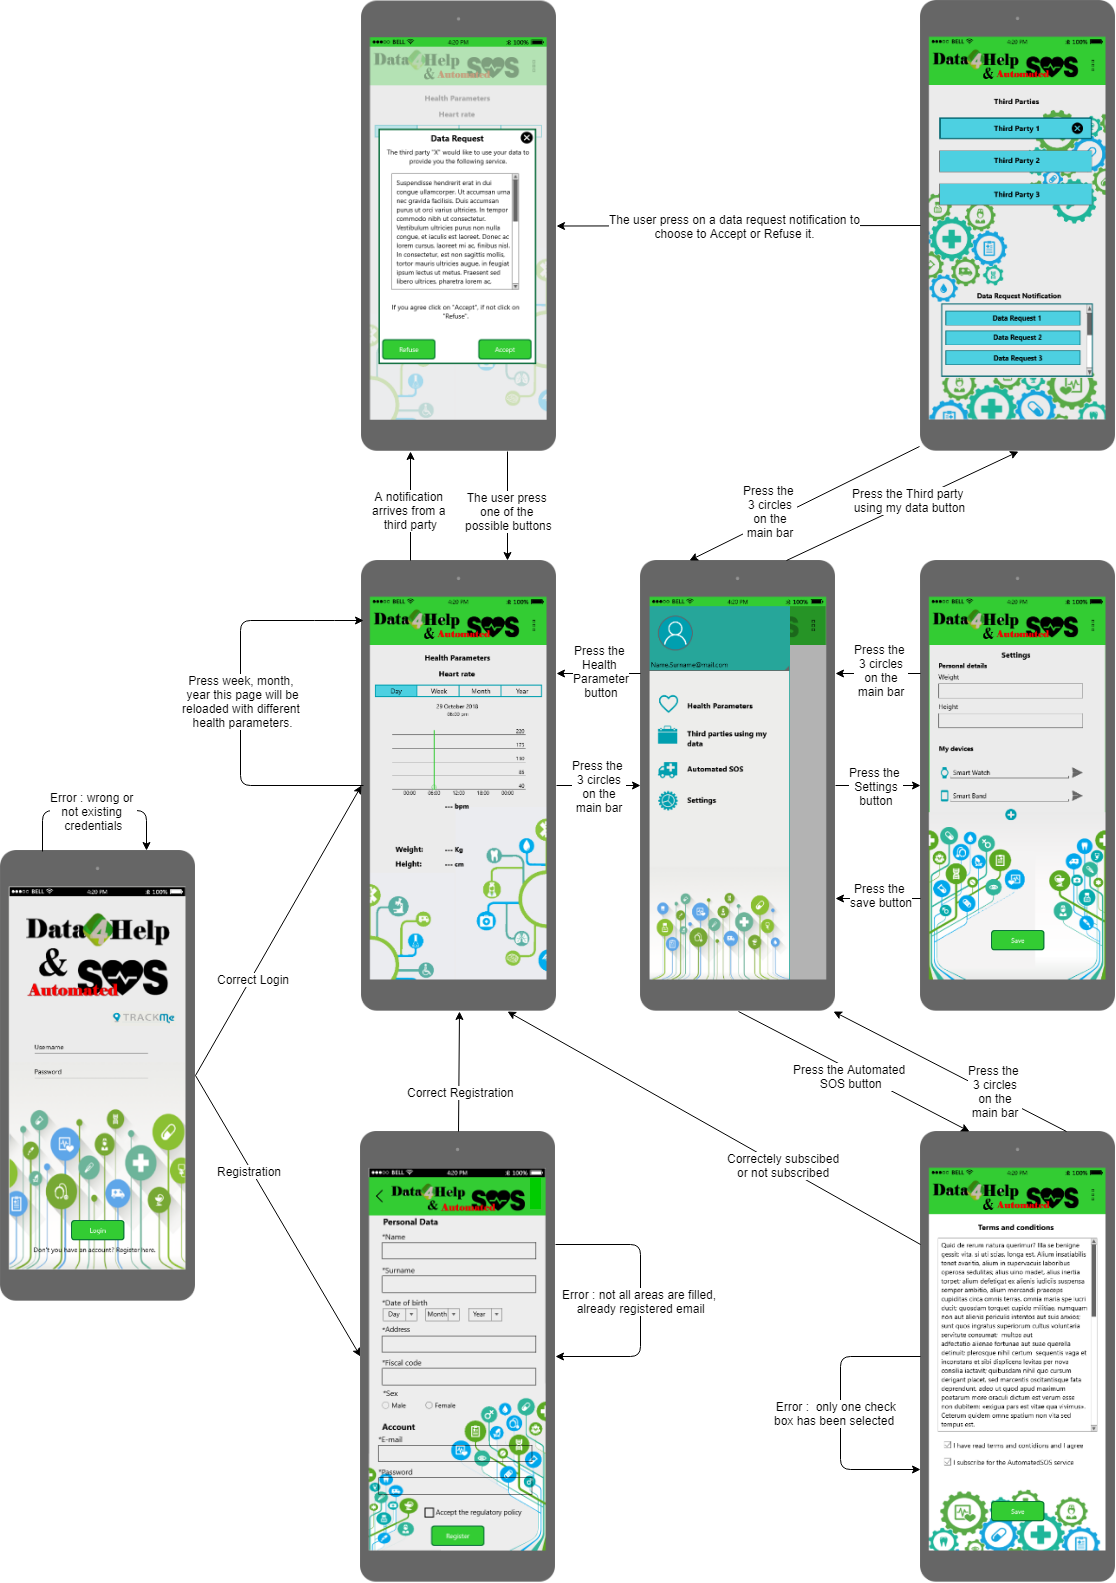
\includegraphics[width=1.0\textwidth]{./pictures/UI_flowchart_diagram.png}\par
	\caption{UI flowchart diagram of the users' mobile app.}
\end{figure}
\FloatBarrier
\begin{figure}[h!]
	\centering
	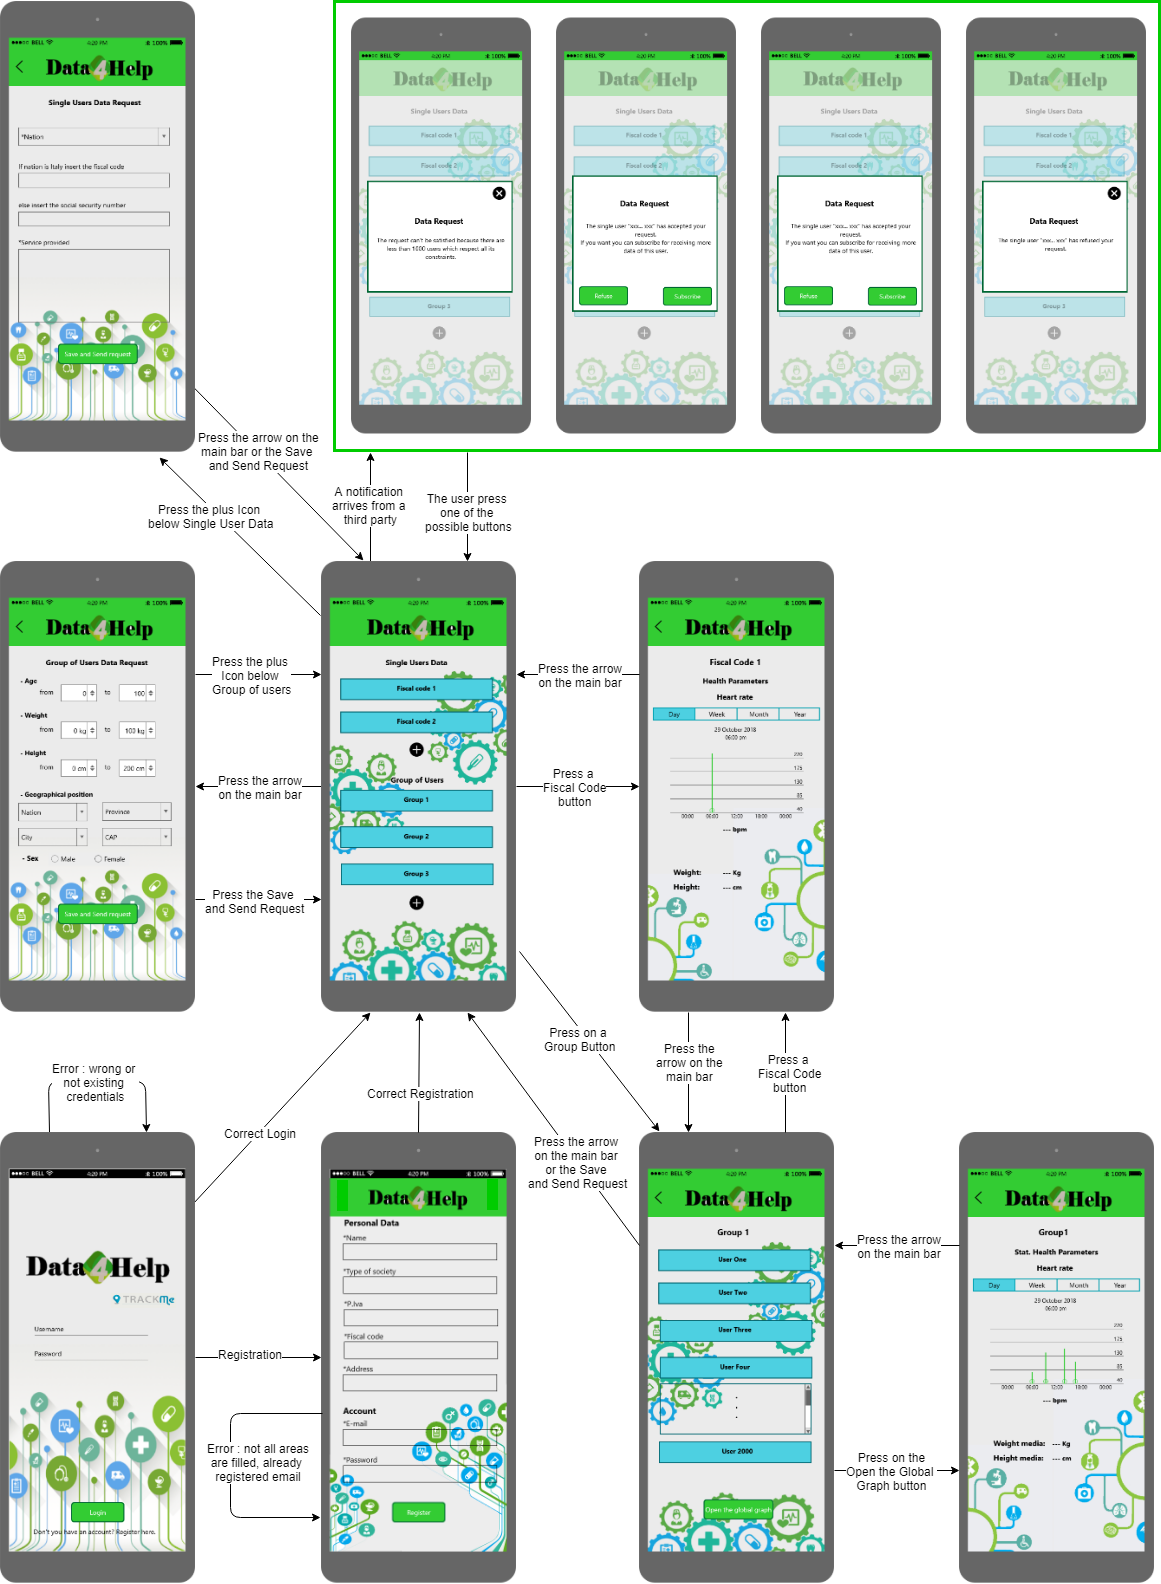
\includegraphics[width=0.90\textwidth]{./pictures/tp_UI_flowchart_diagram.png}\par
	\caption{UI flowchart diagram of the third parties' mobile app. It is equal to the desktop UI flowchart diagram because it does the 		same operation possible on the mobile app.}
\end{figure}
\FloatBarrier
